\chapter{系统总体设计}

\section{系统架构设计}
在构建这套系统时，本研究选取了目前业界比较成熟的 B/S（Browser/Server）架构，并严格按照前后端分离的思路进行模块划分。这样做的目的很明确：一方面是为了保证财务数据在后端逻辑中的安全性，另一方面也方便以后对业务功能进行平滑扩展。

\subsection{技术架构概述}
系统后端是以 Spring Boot 2.6.13 为核心搭建的。开发过程中主要利用了其依赖注入和切面编程特性，把业务逻辑和底层服务彻底解耦，这让代码维护起来没那么吃力。数据持久层则选用了 MyBatis-Plus，配合 Lambda 表达式，既能保证 SQL 的安全性，也省去了写 XML 映射文件的麻烦。前端部分，通过 Vue 3 的组合式 API 和 Element Plus 组件库，系统能够更灵活地构建出那些对响应速度要求较高的交互界面。

\subsection{请求流向的逻辑处理}
为了让数据在各层之间的流动更加有序，笔者为系统设定了一套分层规范。当用户在浏览器端发起一个报销申请时，请求首先会到达表示层，前端在进行基本的输入校验后，会把数据封装成 JSON 报送给后端的 RESTful 接口。

后端的 Controller 层在接收到请求后，会先执行鉴权逻辑，确认无误后再把控制权交给业务逻辑层（Service）。作为系统的“中枢”，Service 层会执行复杂的业务检查，例如在支出记录产生时，程序会调取项目余额并运行多维预警模型。最后，持久层会执行 MyBatis-Plus 生成的 SQL 语句，完成与 MySQL 数据库的交互。这种分层方式虽然增加了一些代码量，但确实显著提升了逻辑的可维护性。

\section{功能模块设计}
根据科研经费管理的业务全貌，系统被拆分成了五个核心模块。

\subsection{用户与权限管理}
安全是财务系统的底座。本设计采用了 RBAC 模型来管理权限，把用户清晰地划分为科研人员和管理员两个层级。在数据存储上，为了防止明文泄密这种低级错误，程序强制要求对密码进行 BCrypt 哈希加密。此外，用户也能在系统里维护自己的资料或修改密码。

\subsection{科研项目全生命周期管理}
这个模块更像是一个驱动业务的状态机。**我**设计了一套包含 6 个状态的流转逻辑，核心在于“节点联动”：比如只有等管理员审核完立项，后续的预算编制功能才会解锁。系统会一直盯着项目的时间进度，这为后面的多维分析提供了必要的时间戳。

\subsection{预算编制与额度控制}
预算管理的核心其实就是“把钱分清楚”。系统引入了科目体系（Fund Category），支持给每个项目分配合理的预算比例。为了防止录入错误，程序内置了一个强校验算法：各科目预算之和必须正好等于批复总额，只要差一分钱，逻辑上就会自动拦截。

\subsection{支出报销与流程审批}
这是经费流动的实际出口，设计遵循的是“余额硬拦截”原则。只要报销金额超过了该科目的当前余额，系统就会自动阻断申报。同时，报销流程也设计了财务初审和复核，每一笔钱花出去都得经过双人审核并留下审计痕迹。

\subsection{多维决策看板}
这是本系统最智能的部分，它依托于数据快照（Snapshot）进行统计。通过 ECharts，原本枯燥的执行率、时间偏差以及科目占比被转化为了直观的图表。笔者设计这一模块的重点在于“主动发现”，系统会自动计算时间进度和经费执行率的差值，帮管理员一眼看出那些执行不力的项目。

\section{数据库设计}

\subsection{数据库概念模型分析}
在设计数据库时，笔者主要围绕科研业务的几个核心实体展开建模。项目负责人与项目之间是一对多的关系，这符合一名老师负责多个项目的实际。而项目则是整个数据网的中心：一个项目对应多个预算科目分配，同时也产生多笔支出流水。

经费科目作为字典基准，它横向贯穿了预算和支出。通过这种关联设计，系统能很方便地把每一笔报销记录归集到对应的科目下，从而实现多维度的聚合统计。这种 E-R 关系（见图 \ref{fig:er_full}）保证了数据的一致性和查询解析的灵活性。

\begin{figure}[htbp]
    \centering
    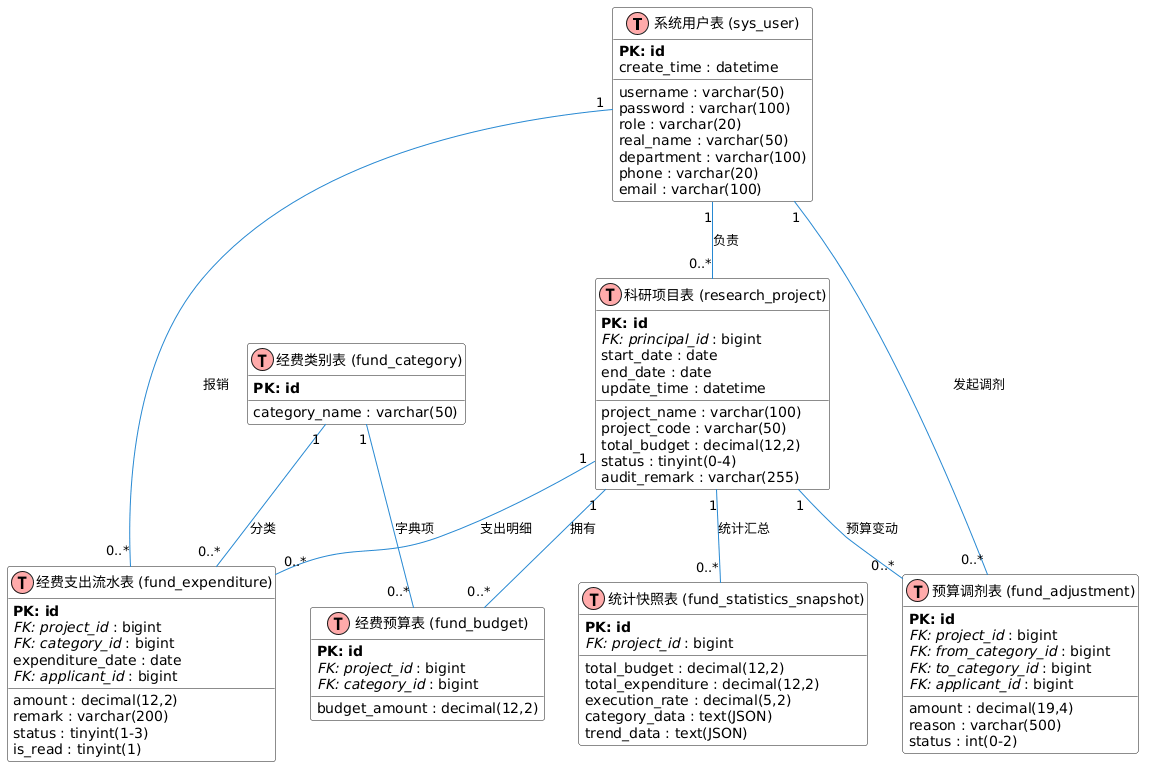
\includegraphics[width=0.9\textwidth]{figures/er-full.png}
    \caption{系统全量 E-R 关系图}
    \label{fig:er_full}
\end{figure}

\subsection{数据库逻辑结构设计}

\begin{table}[htbp]
    \centering
    \caption{系统用户表（sys\_user）结构}
    \label{tab:sys_user}
    \begin{tabular}{|l|l|c|l|}
    \hline
    字段名 & 类型 & 主键 & 说明 \\ \hline
    id & bigint & 是 & 用户内部 ID（自增） \\ \hline
    username & varchar(50) & 否 & 登录用户名 \\ \hline
    password & varchar(100) & 否 & BCrypt 哈希加密密码 \\ \hline
    role & varchar(20) & 否 & 角色（admin/manager/researcher） \\ \hline
    real\_name & varchar(50) & 否 & 真实姓名 \\ \hline
    department & varchar(100) & 否 & 所属学院/部门 \\ \hline
    phone & varchar(20) & 否 & 联系电话 \\ \hline
    email & varchar(100) & 否 & 电子邮箱 \\ \hline
    create\_time & datetime & 否 & 注册时间 \\ \hline
    \end{tabular}
\end{table}

\begin{table}[htbp]
    \centering
    \caption{科研项目表（research\_project）结构}
    \label{tab:research_project}
    \begin{tabular}{|l|l|c|l|}
    \hline
    字段名 & 类型 & 主键 & 说明 \\ \hline
    id & bigint & 是 & 项目 ID \\ \hline
    project\_name & varchar(100) & 否 & 项目全称 \\ \hline
    project\_code & varchar(50) & 否 & 财务项目编号 \\ \hline
    principal\_id & bigint & 否 & 负责人 ID \\ \hline
    start\_date & date & 否 & 开始时间 \\ \hline
    end\_date & date & 否 & 结束时间 \\ \hline
    total\_budget & decimal(12,2) & 否 & 项目总预算 \\ \hline
    status & tinyint & 否 & 状态（0-草稿/1-待审/2-立项/3-驳回等） \\ \hline
    audit\_remark & varchar(255) & 否 & 审批意见/驳回原因 \\ \hline
    update\_time & datetime & 否 & 数据最后更新时间 \\ \hline
    \end{tabular}
\end{table}

\begin{table}[htbp]
    \centering
    \caption{经费科目表（fund\_category）结构}
    \label{tab:fund_category}
    \begin{tabular}{|l|l|c|l|}
    \hline
    字段名 & 类型 & 主键 & 说明 \\ \hline
    id & bigint & 是 & 科目 ID \\ \hline
    category\_name & varchar(50) & 否 & 科目名称 \\ \hline
    \end{tabular}
\end{table}

\begin{table}[htbp]
    \centering
    \caption{经费预算表（fund\_budget）结构}
    \label{tab:fund_budget}
    \begin{tabular}{|l|l|c|l|}
    \hline
    字段名 & 类型 & 主键 & 说明 \\ \hline
    id & bigint & 是 & 预算项 ID \\ \hline
    project\_id & bigint & 否 & 项目 ID \\ \hline
    category\_id & bigint & 否 & 经费类别 ID \\ \hline
    budget\_amount & decimal(12,2) & 否 & 分项核定预算金额 \\ \hline
    \end{tabular}
\end{table}

\begin{table}[htbp]
    \centering
    \caption{经费支出记录表（fund\_expenditure）结构}
    \label{tab:fund_expenditure}
    \begin{tabular}{|l|l|c|l|}
    \hline
    字段名 & 类型 & 主键 & 说明 \\ \hline
    id & bigint & 是 & 记录 ID \\ \hline
    project\_id & bigint & 否 & 项目 ID \\ \hline
    category\_id & bigint & 否 & 经费类别 ID \\ \hline
    amount & decimal(12,2) & 否 & 报销金额 \\ \hline
    expenditure\_date & date & 否 & 支出实际日期 \\ \hline
    status & tinyint & 否 & 状态（1-待审/2-通过/3-驳回） \\ \hline
    applicant\_id & bigint & 否 & 申请报销人 ID \\ \hline
    is\_read & tinyint(1) & 否 & 消息是否已读 \\ \hline
    \end{tabular}
\end{table}

\begin{table}[htbp]
    \centering
    \caption{预算调剂表（fund\_adjustment）结构}
    \label{tab:fund_adjustment}
    \begin{tabular}{|l|l|c|l|}
    \hline
    字段名 & 类型 & 主键 & 说明 \\ \hline
    id & bigint & 是 & 调剂记录 ID \\ \hline
    project\_id & bigint & 否 & 关联项目 ID \\ \hline
    from\_category\_id & bigint & 否 & 调出科目 ID \\ \hline
    to\_category\_id & bigint & 否 & 调入科目 ID \\ \hline
    amount & decimal(19,4) & 否 & 调剂金额（高精度） \\ \hline
    status & int & 否 & 状态（0-待审/1-通过/2-驳回） \\ \hline
    applicant\_id & bigint & 否 & 调剂发起人 ID \\ \hline
    \end{tabular}
\end{table}

\begin{table}[htbp]
    \centering
    \caption{经费统计快照表（fund\_statistics\_snapshot）结构}
    \label{tab:fund_statistics_snapshot}
    \begin{tabular}{|l|l|c|l|}
    \hline
    字段名 & 类型 & 主键 & 说明 \\ \hline
    id & bigint & 是 & 快照 ID \\ \hline
    project\_id & bigint & 否 & 项目 ID \\ \hline
    execution\_rate & decimal(5,2) & 否 & 实时经费执行率 \\ \hline
    category\_data & text & 否 & 分类占比 JSON 数据 \\ \hline
    trend\_data & text & 否 & 趋势分析 JSON 数据 \\ \hline
    \end{tabular}
\end{table}

\begin{table}[htbp]
    \centering
    \caption{系统日志表（sys\_log）结构}
    \label{tab:sys_log}
    \begin{tabular}{|l|l|c|l|}
    \hline
    字段名 & 类型 & 主键 & 说明 \\ \hline
    id & bigint & 是 & 日志 ID \\ \hline
    user\_id & bigint & 否 & 操作用户 ID \\ \hline
    action & varchar(200) & 否 & 业务操作行为 \\ \hline
    ip\_address & varchar(45) & 否 & 访问 IP 地址 \\ \hline
    create\_time & datetime & 否 & 操作发生时间 \\ \hline
    \end{tabular}
\end{table}

\section{本章小结}
本章详尽论述了系统的总体设计方案。在确立前后端分离架构的基础上，笔者进一步对业务流向进行了逻辑分层，确保了核心业务处理的有序性。通过对五个核心功能模块的拆解，明确了项目、预算和支出的管控策略。最后，通过 E-R 模型和物理表设计，完成了底层的数据库建模。这些设计环节共同构成了系统的开发蓝图，为接下来的具体实现提供了明确的代码参照。
